\documentclass[conference]{IEEEtran}
\IEEEoverridecommandlockouts

\usepackage{cite}
\usepackage{amsmath,amssymb,amsfonts}
\usepackage{algorithmic}
\usepackage{graphicx}
\usepackage{textcomp}
\usepackage{xcolor}
\def\BibTeX{{\rm B\kern-.05em{\sc i\kern-.025em b}\kern-.08em
    T\kern-.1667em\lower.7ex\hbox{E}\kern-.125emX}}

\begin{document}

\title{Assignment 2}

\author{Tingjun Yuan}

\maketitle

\begin{abstract}
This assignment is mainly based on the knowledge of Attention Mechanisms and
Graph Neural Networks (GNN). The dataset is generally based on a pedestrian
trajectory recorded in a mall. The models trained in the assignment predict
the positions of the pedestrians. This assignment first trains a GNN model
according to a tutorial, but reimplemented with PyTorch. After training, the
model is evaluated with the main squared error (MSE), the mean Euclidean
distance, and the plot graphs. Next, the model is reexamined by tuning
hyperparameters, trying a deeper embedding, and replacing the learned attention
mechanism. This report shows the results of the model evaluation and discusses
them.
\end{abstract}

\section{Result and Evaluation}

\subsection*{Task 1}

This task preprocesses the data, defines the classes for layers and training
logic, trains the model, and evaluates it by calculating the mean squared error
(MSE) and visualizing the differences between prediction and real future
positions. This step follows the tutorial \cite{cite:tut} and rewrites the code
using PyTorch, another deep learning library which is more compatible with the
experiment environment.

The hyperparameters for the training is as follows:

\begin{verbatim}
    hidden_units=100,
    num_heads=8,
    num_layers=3,
    output_dim=2,
    num_epochs=100,
    learning_rate=1e-3,
\end{verbatim}

After training the model with 100 epochs, the training MSE is \textbf{0.4717},
and the test mean Euclidean distance is \textbf{0.1763}. In addition, one of
the scenes is randomly chosen from the test set to perform evaluation by
visualizing the coordinates. The result is shown in Figure~\ref{fig:visual1}.

\begin{figure}[htbp]
    \centering
    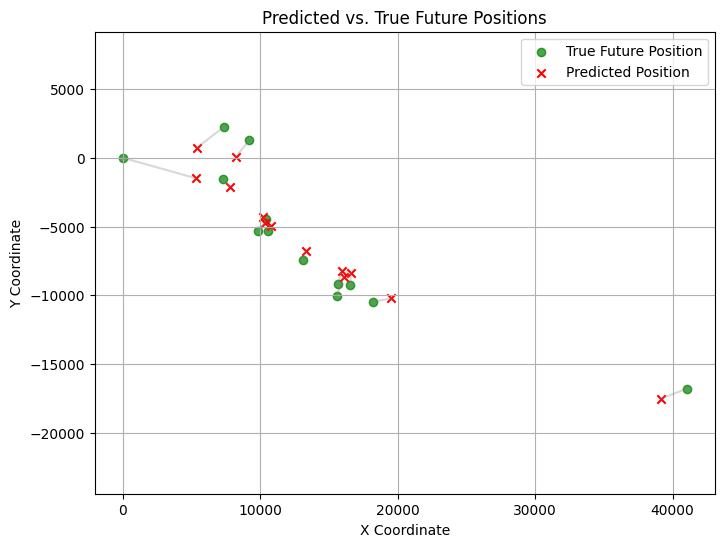
\includegraphics[width=0.8\linewidth]{figvisual1.png}
    \caption{Visualization on the Original Model}
    \label{fig:visual1}
\end{figure}

\subsection*{Task 2}

This task consists of two parts: performing hyperparameter tuning of the number
of attention heads, and trying a deeper embedding of the node features. 

\begin{thebibliography}{00}
\bibitem{cite:tut} A. Kensert, “Graph attention network (GAT) for node
    classification,” 2021, Keras. [Online]. Available:
    https://keras.io/examples/graph/gat\_node\_classification/
\end{thebibliography}

\end{document}
